%!TEX root = ../../Paper.tex

\chapter{Foundations}
\label{cha:foundations}

\section{Performance and Metrics}
\label{sec:performance-metrics}
Certain applications fail to meet specific performance requirements which results in the damage of customer relations, less productive users, lower revenues or an explosion of maintenance costs \cite{smith.1998}. This chapter specifies how performance is quantified using so called performance metrics.

Metrics create a uniform understanding of how to interpret measurements. They make it possible to compare various measurements across different series and systems. Lilja describes the following characteristics of a computer system which should be considered in this context \cite[9]{lilja.2005}:

\begin{itemize}
  \item the occurrence frequency of an event
  \item the duration of an event
  \item the size of a parameter
\end{itemize}

These characteristics can directly be used as a metric or like in most cases be transferred to a standardised scale and observed in a bounded time interval \cite[9]{lilja.2005}. Most of the metrics are evaluated by taking the average of a measurement series. In some cases it can be of interest to evaluate the minimum or maximum value of a measurement series \cite[48]{jain.2008}. Hence it is recommended to always specific which characteristic of a metric is being evaluated.

\subsection*{Response time}
The response time $RT$ is a universal performance metric which is widely used when describing the performance of a system \cite{lilja.2005, cortellessa.2007}. When using the response time as a metric it is important to specify which what is described with the results. The response time can be used to describe whole transactions as the sum of response times of multiple methods being executed in a series. On the other it is possible to describe the duration the single operations inside a method. Independently from the level of abstraction the lower is better applies to the response time metric \cite[54]{jain.2008}. The metric is specified in any consistent time unit which is in most cases seconds or milliseconds. It is computed as the difference from the end point $t_{end}$ and start point $t_{start}$ of the measurement:

\[
  RT = t_{end} - t_{start} .
\]

The throughput \large{$\tau$}\normalsize{} of an element (transaction, method, operation, etc.) is described using the response time. It is defined as the count of action per time unit $\Delta t$\footnote{In most cases the throughput is evaluated as actions per second so $\Delta t = 1s$} \cite[19]{lilja.2005}. The formula to calculate the throughput from the response time $RT$ is defined as follows:

\[
  \mathlarger{\tau} = \frac{\Delta t}{RT} .
\]

\subsection*{System utilization}
System utilization is a generic term for all metrics describing the utilization of the \acf{SUT} \cite[48]{jain.2008}. The term includes among others the processor utilization, network utilization, internal memory utilization or the disk utilization. The values are specified in percentage to make them comparable independently from the unit of measurement or their cardinality. There is no general applicable predicate which utilization is ideal (nominal is best) \cite[54]{jain.2008}. A system which is never fully utilized could be a sign for oversized architecture for the given task. Whereas an system which runs on full load the whole time could perform better with more available resources. For different components of an application different system utilization metrics are relevant. A database server is best described by disk or internal memory utilization hence the application server executing the intensive business logic is possibly better described by the processor utilization.

\section{Workload Types}
\label{sec:workloads}
Schroeder et al. define three different types of workloads: the close, the open and the partly-open workload (cf.~figure~\ref{fig:workload-types}) \cite{Schroeder.2006}. A closed workload assumes that there is a fixed number of users who use the \ac{SUT} forever. The users complete a specified task on the system and wait for a predefined time, the so called think time, and start the task over again \cite[3]{Schroeder.2006}. In contrast in an open system there is a stream of users which complete task and disappear afterwards. So new requests are not triggered by a previous job completion \cite[3]{Schroeder.2006}. Since neither the closed nor the open workload are very realistic Schroeder et al. came up with the partly-open workload as an alternative. It consists out of a stream of new arriving users (like the open workload) which execute with a defined probability of $\rho$ another task on the \ac{SUT} (like the closed workload) \cite[3 - 4]{Schroeder.2006}.

\begin{figure}[h]
  \centering
  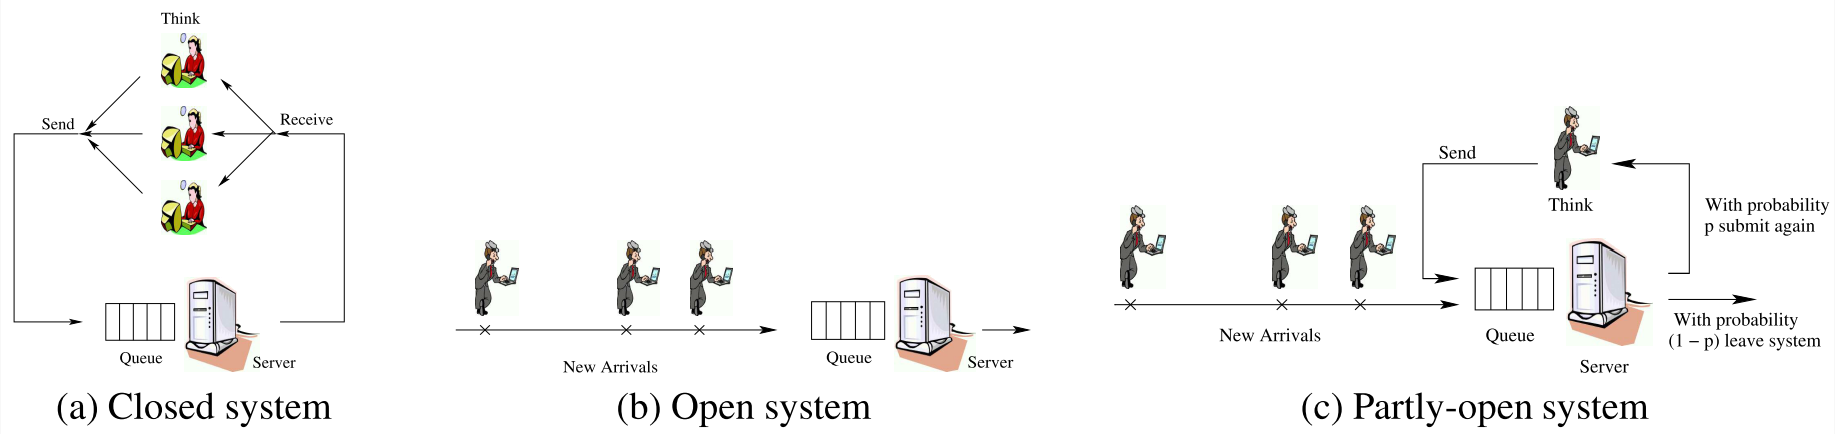
\includegraphics[width=\textwidth]{Figures/workload_types.png}
  \caption[Workload types]{Workload types}
  \label{fig:workload-types}
\end{figure}

It is important to define which kind of workload a benchmark is using to be able to conduct comparable and repeatable experiments. In addition to the workload type the workload mix plays an important role. It defines what kind of actions each users does in the \ac{SUT}. The easiest workload mix is achieved by setting a probability for read and for write request on the database. Another approach would be to define the workload mix very accurate and application driven. By observing the users of an existing application usage profiles are created which then are used to describe the workload mix. In the real-world a decision has to be made for the trade-off between a quickly defined and implemented workload mix or a more accurate, usage driven approach.

\section{Distributed Cloud Computing}
\label{sec:distributed-computing}
Distributed computing describes the segmentation of computing power from one processor core on one physical machine to multiple cores on various machines. An outstanding example for the advantages of distributed computing is the raising trend of cloud computing. Users do not have the massive computing power needed to solve today's complex problems in their home or business but rather outsource it in cloud. By utilizing \acf{PaaS} and \acf{IaaS} they only need a lightweight device to access their data and applications instead of a full fledged computer. \cite[1 - 2]{dikaiakos.2009}

There are three different types of clouds. The first one is the so called \emph{private cloud} which is hosted by a single organization or group. The second is available to the public (\emph{public cloud}) and the is the \emph{hybrid cloud} which is hosted by multiple organizations or groups. All clouds have in common that they automatically scale up as the loads on the machines increases (\emph{elasticity}). Most of the public clouds have a so called pay-as-you-go economic model where only the consumer has only to pay for the computing power it actually uses. \cite[2]{dikaiakos.2009}


\section{NoSQL}
\label{sec:nosql}
\acf{NoSQL} describes a group of non relation data management systems which in most cases do not use \acf{SQL} as data manipulation language \cite[1]{moniruzzaman.2013}. \ac{NoSQL} systems are usually distributed databases used to store large-scale data and perform parallel data analysis. They are used when traditional relational databases reach their limit for example when dealing with a huge amount of different entity types. \cite[1 - 2]{moniruzzaman.2013} \cite[23]{orend.2010}

NoSQL databases can be differentiated by their underlying data model. The most widespread data models are categorized as follows \cite[34]{ellis.2010} \cite[2 - 3]{hecht.2011}:

\begin{itemize}
  \item Document Stores
    \begin{itemize}
      \item CouchDB \cite{couch.2014}, MongoDB \cite{mongo.2014}, Riak \cite{riak.2014}
    \end{itemize}
  \item Column Family Stores
    \begin{itemize}
      \item Google Bigtable \cite{chang.2006}, Cassandra \cite{cassandra.2014}, HBase \cite{hbase.2014}, Hypertable \cite{hypertable.2014}
    \end{itemize}
  \item Graph databases
    \begin{itemize}
      \item Neo4j \cite{neo4j.2014}, FlockDB \cite{flock.2010}, AllegroGraph \cite{allegro.2014}
    \end{itemize}
  \item Key-Value Stores
    \begin{itemize}
      \item Memcached \cite{memcached.2014}, Project Voldemort \cite{voldemort.2013}, Redis \cite{redis.2014}, 
    \end{itemize}
\end{itemize}

\subsection{ACID}
\label{subsec:acid}
Relational databases provide as opposed to \ac{NoSQL} databases full ACID support to ensure that transaction are executed reliably. ACID is an acronym for Atomicity, Consistency, Isolation and Durability. Where atomicity defines that any transaction has to be fully executed or otherwise is reversed. Consistency ensures that are each transaction only produces valid data and do not corrupt any table. Isolation implies that no transaction influences another or distorts another results. Finally durability describes that no data will be lost when there is a system failure. \cite[71]{pokorny.2011}

ACID properties are most of the time ensured by introducing locking-mechanism which influence the performance negatively \cite[1]{hecht.2011}. NoSQL databases do not support full ACID properties hence introducing eventually consistency. The concept behind the trade-off between being strongly consistent and a higher availability and greatly improved scalability is evaluated in the next section.


\subsection{CAP}
\label{subsec:cap}
CAP is an acronym for Consistency, Availability and Partition tolerance. Consistency means that every read from the database returns the latest data, which is different from the consistency definition of the ACID properties. Availability ensures that every query on the databases is answered as fast as possible and no query gets lost. This is most of the time achieved by utilizing many physical machines and distributed load between them. Partition tolerance implies that the data saved on a node is duplicated on multiple other nodes making sure that when a node failed to respond to a request the request is forwarded to a node which is able to respond. \cite[72]{pokorny.2011}

\begin{figure}[H]
  \centering
  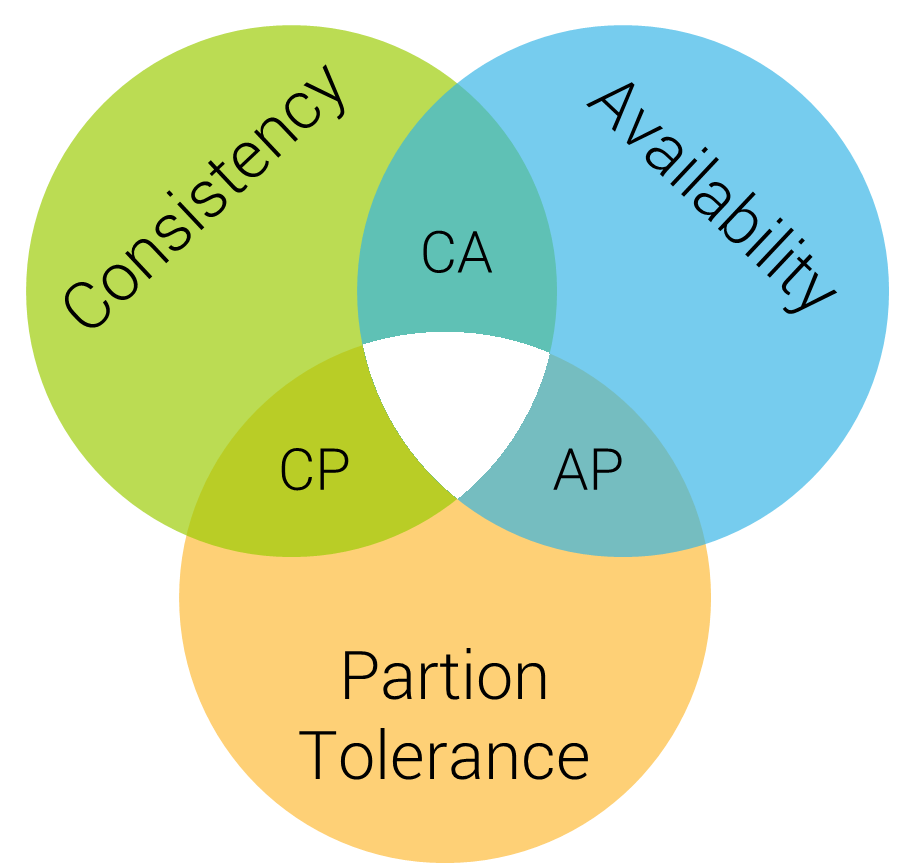
\includegraphics[width=.4\textwidth]{Figures/cap.png}
  \caption[CAP Theorem]{CAP Theorem}
  \label{fig:cap-theorem}
\end{figure}

The CAP or Brewer's theorem describes that it is impossible to guarantee all the properties at the same time. There will always be a trade off which has to be evaluated for every use case (cf.~figure~\ref{fig:cap-theorem}). Choosing AP (Availability and Partition tolerance) over CA (Consistency and Availability) does not mean that the database is not consistent at all, but that it does not focus on being strongly consistent to serve incoming requests faster. Most of the NoSQL database have given up being strongly consistent in order to gain a higher availability and better partition tolerance, this is sometimes called BASE (Basically Available, Soft-state, Eventually consistent) \cite[4]{moniruzzaman.2013}.